\documentclass[../main.tex]{subfiles}

\begin{document}

\section{Exploring the AHEAD brains together}

\authors{Alessandra Pizzuti\textsuperscript{1}, Sebastian Dresbach\textsuperscript{1}, Satrajit Ghosh\textsuperscript{2}, Katja Heuer\textsuperscript{3}, Roberto Toro\textsuperscript{3}, Pierre-Louis Bazin\textsuperscript{4,5}}

\affiliations{1. Maastricht University, Maastricht, Netherlands; 2. Massachussetts Institute of Technology, Boston, USA; 3. Institut Pasteur, Paris, France; 4. University of Amsterdam, Amsterdam, Netherlands; 5. Max Planck Institute for Human Cognitive and Brain Science, Leipzig, Germany.}

\subsection{Introduction}
One of the long-standing goals of neuroanatomy is to compare the cyto- and myeloarchitecture of the human brain. The recently made available 3D whole-brain post-mortem data set provided by \textcite{Alkemade2022} includes multiple microscopy contrasts and 7-T quantitative multi-parameter MRI reconstructed at 200µm from two human brains. Through the co-registration across MRI and microscopy modalities, this data set provides a unique direct comparison between histological markers and quantitative MRI parameters for the same human brain. In this BrainHack project, we explored this dataset, focusing on: (i) data visualization in online open science platforms, (ii) data integration of quantitative MRI with microscopy, (iii) data analysis of cortical profiles from a selected region of interest. 


\subsection{Results}

Visualization and annotation of large neuroimaging data sets can be challenging, in particular for collaborative data exploration. Here we tested two different infrastructures: BrainBox \url{https://brainbox.pasteur.fr/}, a web-based visualization and annotation tool for collaborative manual delineation of brain MRI data, see e.g. \parencite{heuer_evolution_2019}, and Dandi Archive \url{https://dandiarchive.org/}, an online repository of microscopy data with links to Neuroglancer \url{https://github.com/google/neuroglancer}. While Brainbox could not handle the high resolution data well, Neuroglancer visualization was successful after conversion to the Zarr microscopy format (fig.~\ref{fig:ahead}A).

To help users explore the original high-resolution microscopy sections, we also built a python notebook to automatically query the stains around a given MNI coordinate using the Nighres toolbox~\parencite{huntenburg_nighres_2018} (fig.~\ref{fig:ahead}B).

For the cortical profile analysis we restricted our analysis on S1 (BA3b) as a part of the somato-motor area from one hemisphere of an individual human brain. S1 is rather thin (\(\sim\)2mm) and it has a highly myelinated layer 4 (see arrow fig.~\ref{fig:test}C). In a future step, we are aiming to characterize differences between S1 (BA3b) and M1 (BA4). For now, we used the MRI-quantitative-R1 contrast to define, segment the region of interest and compute cortical depth measurement. In ITK-SNAP \parencite{Yushkevich2006} we defined the somato-motor area by creating a spherical mask (radius 16.35mm) around the ‘hand knob’ in M1. To improve the intensity homogeneity of the qMRI-R1 images, we ran a bias field correction (N4BiasFieldCorrection, \parencite{Cox1996}). Tissue segmentation was restricted to S1 and was obtained by combining four approaches: (i) fsl-fast \parencite{Smith2004} for initial tissues probability map, (ii) semi-automatic histogram fitting in ITK-SNAP, (iii) Segmentator \parencite{Gulban2018}, and (iv) manual editing. We used the LN2\_LAYERS program from LAYNII open source software \parencite{Huber2021}  to compute the equi-volume cortical depth measurements for the gray matter. Finally, we evaluated cortical depth profiles for three quantitative MRI contrasts (R1, R2, proton density) and three microscopy contrasts (thionin, bieloschowsky, parvalbumin) by computing a voxel-wise 2D histogram of image intensity (fig.~\ref{fig:test}C). Some challenges are indicated by arrows 2 and 3 in the lower part of fig.~\ref{fig:test}C.

From this Brainhack project, we conclude that the richness of the data set must be exploited from multiple points of view, from enhancing the integration of MRI with microscopy data in visualization software to providing optimized multi-contrast and multi-modality data analysis pipeline for high-resolution brain regions.

\printbibliography


\begin{figure*}
	\centering
	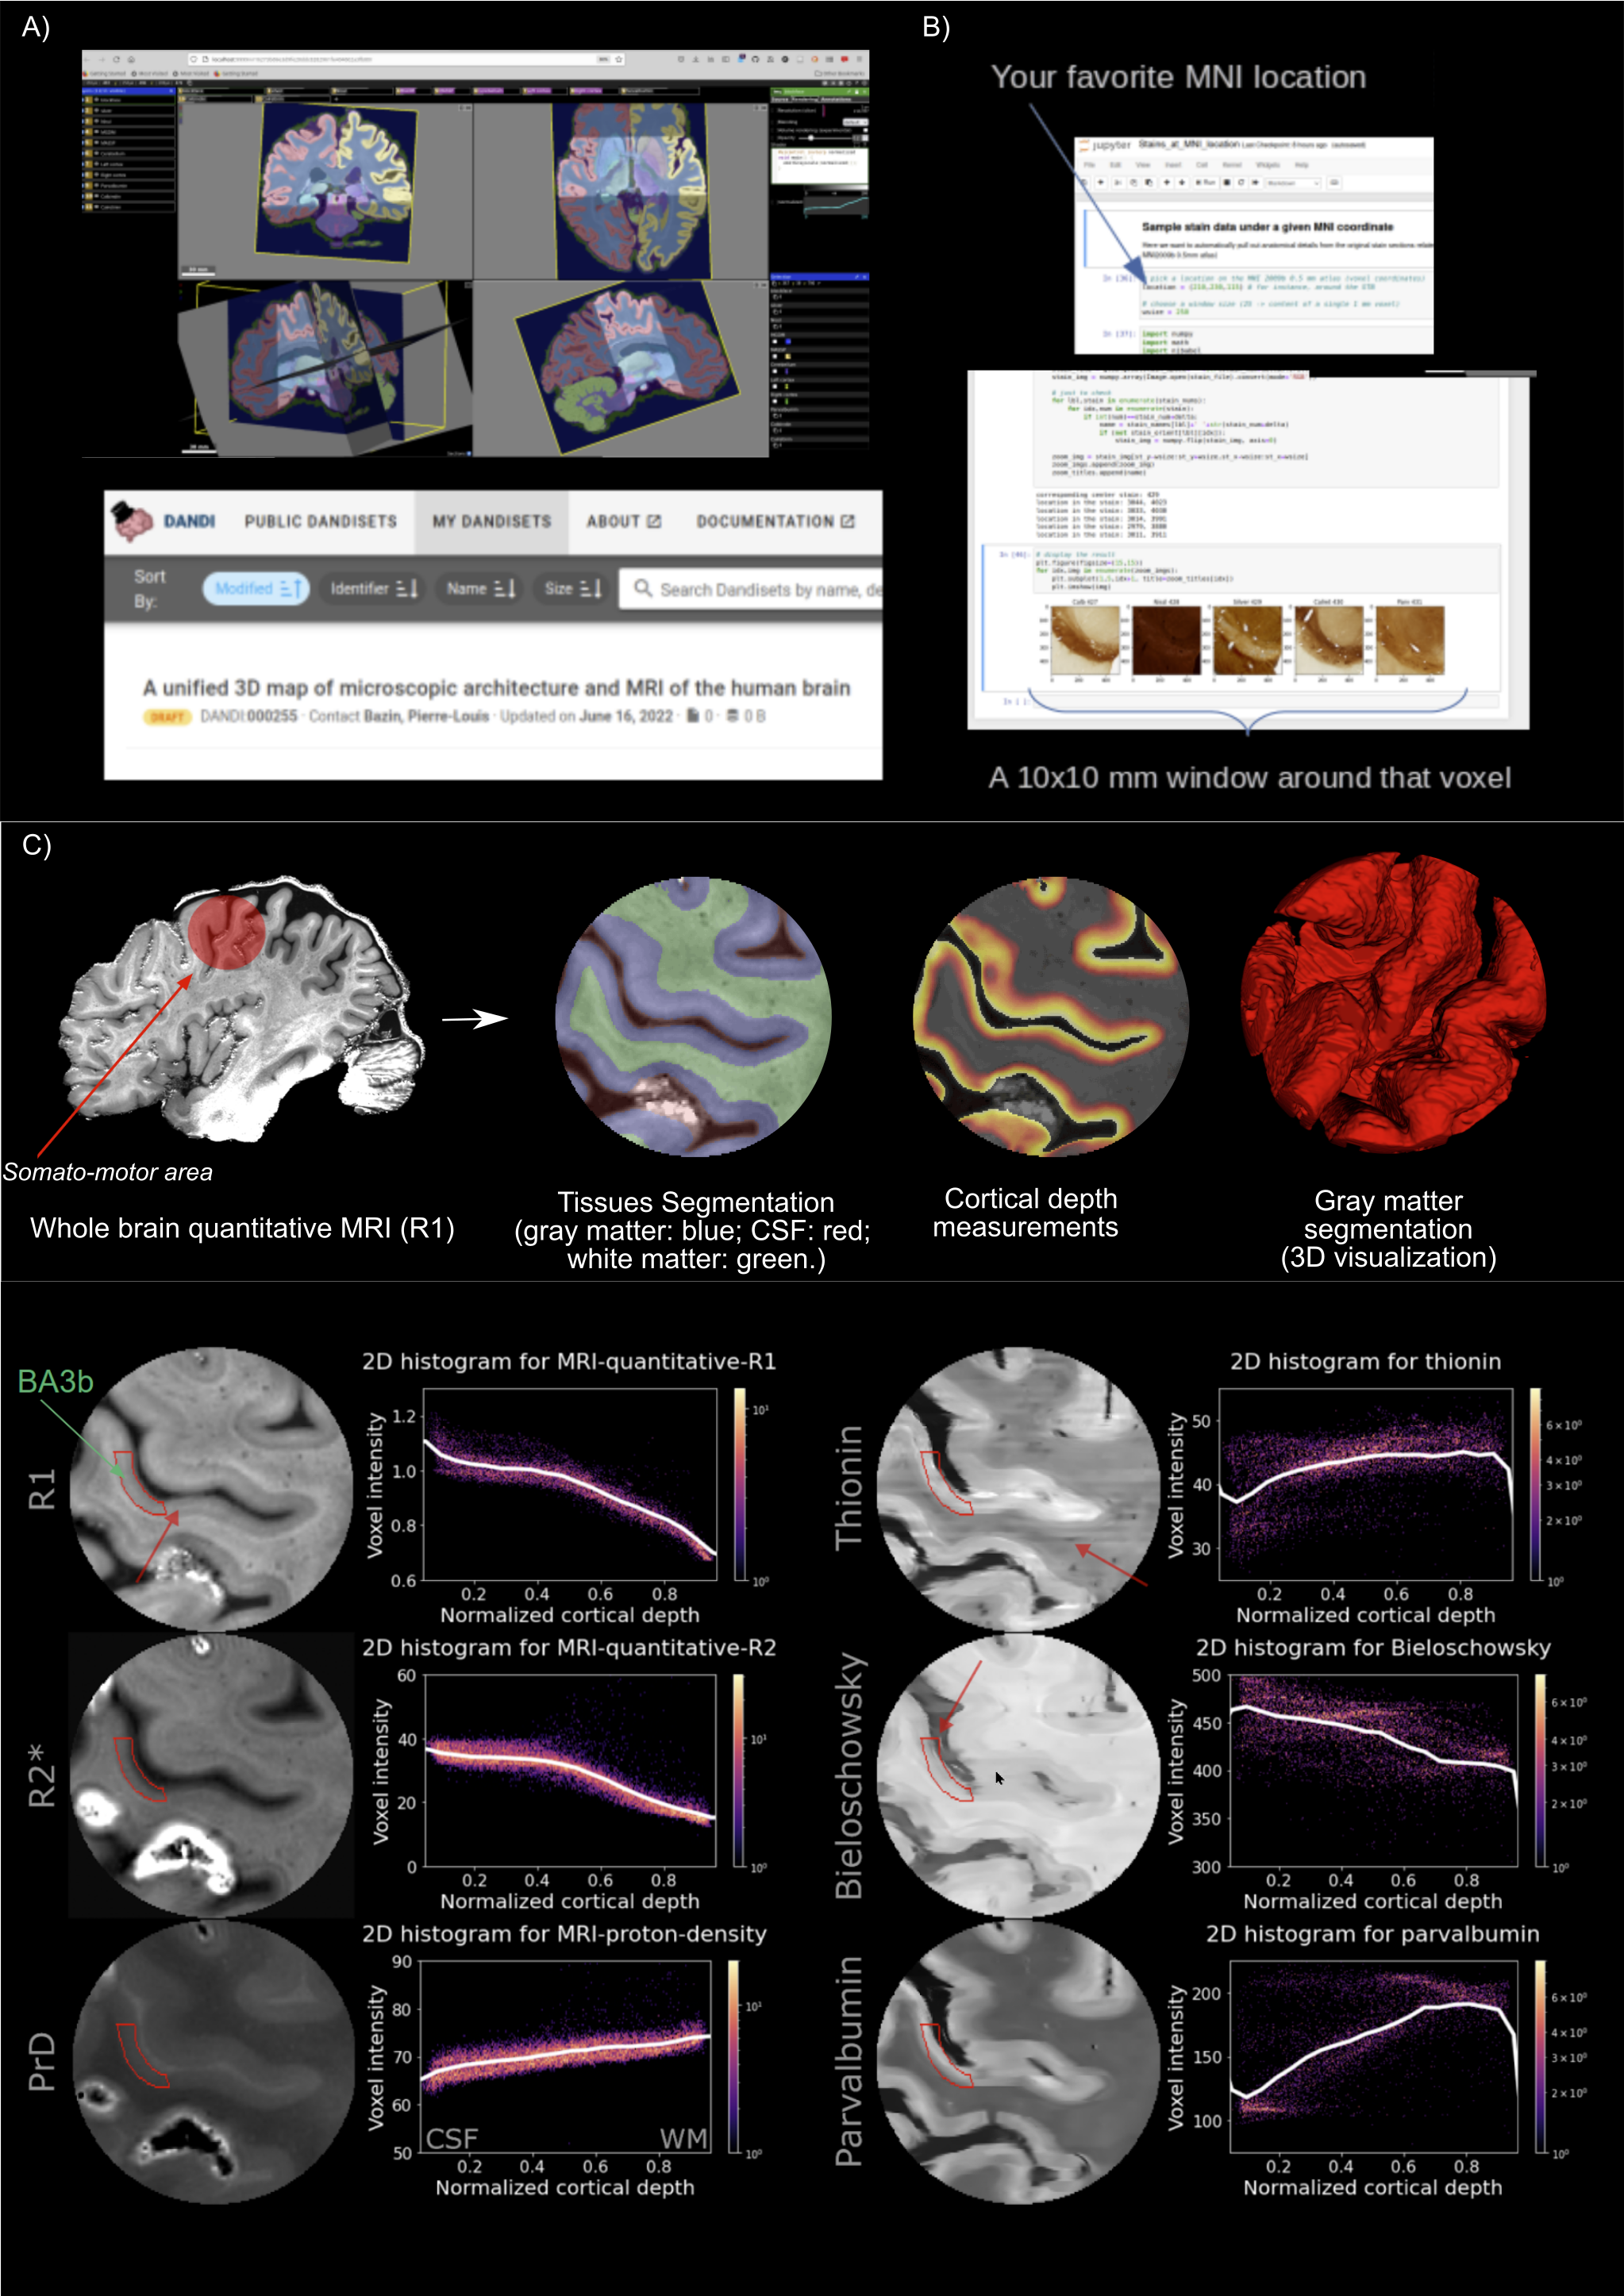
\includegraphics[width=1\textwidth]{AHEAD_Figure_1.png}
	\caption{A) Neuroglancer visualization, B) section query notebook, C) Cortical ROI and corresponding depth histograms extracted from the different contrasts available.
	}
	\label{fig:ahead}
\end{figure*}


\end{document}
